 A basic event selection is made for selecting signal like events and is discussed in \Sec{sec:trig}. Also the effect corrections applied to simulation and data, summarised in \Sec{sec:SummaryCor} is shown. The analysis strategy is presented in \Sec{sec:selection}, defining the signal and background regions to constrain the huge \SM\ background compared to the expected signal. \Sec{sec:regions} discusses each region that is entering the analysis. On top of the use of background estimation from control regions, backgrounds that have  prompt leptons  contaminated by real leptons either
from decays of tau leptons or from hadronized mesons or baryons
(collectively commonly referred as ``non-prompt leptons") as well as by
hadrons or jets misidentified as leptons\footnote{These two classes
	of contamination will be referred to as not prompt-lepton (\NPL) samples.} are
evaluated with a data-driven method discussed in \Sec{sec:NPL}.

\section{Baseline event selection and filters}
\label{sec:trig}
 In this analysis a search is performed in a final state made up of a \PZ\ boson and a top quark, associated or not with a jet, in the leptonic decay of the \PZ\ boson and the top quark. The leading order Feynman diagrams can be seen in \fig{fig:feynST} and \fig{fig:feynTT}. 
 The signal considers both the single top quark \FCNC\ (\tZ\ in the final state) and the top quark pair \FCNC\ (\tZq\ with $\Pquark= \Pcharm, \Pup$ in the final state) events. Their final state signatures consist of three leptons, considering electrons or muons, and a jet originating from a \Pbottom\ quark. For \FCNC\ \tZq, there is an additional up or charm jet. Leptons from tau decays are not vetoed and are entering the analysis via their leptonic decays. Four different lepton channels based on lepton flavour are considered: \eee, \eemu, \emumu, and \mumumu.
\begin{figure}[htbp]
	\centering
	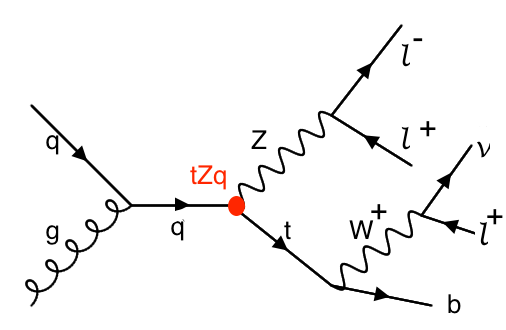
\includegraphics[width=0.45\linewidth]{5_EventSelection/Figures/feynmanST}
	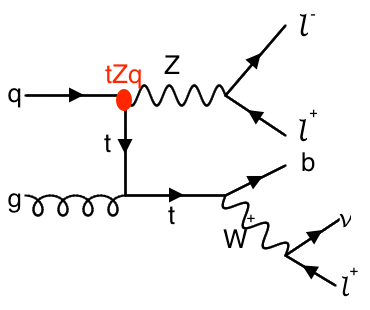
\includegraphics[width=0.35\linewidth]{5_EventSelection/Figures/FeynmanSTtzq}
	\caption{Single top quark Feynman diagrams at leading order. The vertex labelled \tZq\ is the sought-for \FCNC\ interaction.}
	\label{fig:feynST}
\end{figure}
\begin{figure}[htbp]
	\centering
	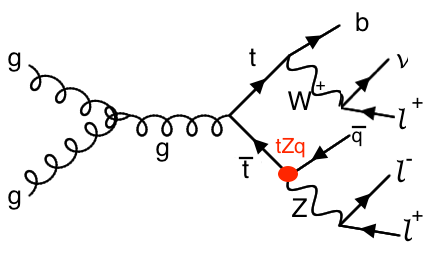
\includegraphics[width=0.45\linewidth]{5_EventSelection/Figures/FeynmantttZq}
	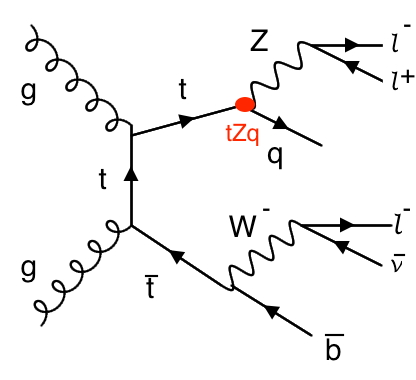
\includegraphics[width=0.35\linewidth]{5_EventSelection/Figures/FeynmantttZq2}
	\caption{Top quark pair Feynman diagram at leading order. The vertex labelled \tZq\ is the sought-for \FCNC\ interaction. }
	\label{fig:feynTT}
\end{figure}
  

The CMS collaboration recorded in the course of 2016 proton at 13 \TeV\ collisions data with a total recorded integrated luminosity of $35.9~\fbinv$. The baseline event selection has a goal to substantially reject \SM\ background events, whilst maintaining a high signal efficiency. The CMS trigger system, described in \Sec{sec:DAQ}, filters out the main of the collision events from uninteresting processes and dedicated trigger paths are defined to single out the events with our required detector signature. The trigger paths are chosen based on on-line triggering objects with at least one muon (M), at least one electron (E), at least two muons (MM), at least two electrons (EE), at least one muon and an electron (ME), at least three muons (MMM), at least three electrons (EEE), at least two muons and one electron (MME), or at least two electrons and one muon (EEM). For the MC simulation a simple $or$ of all triggers is taken and the event is considered when it passes one of the trigger paths. For data however, double counting of the same event has to be taken into account and a procedure to avoid double counting has been put into place. It consists of vetoing in a given dataset the events that are already selected in another, as given in Table \ref{tab:triggerlogic}. 
\begin{table}[htbp]
	\centering
	\caption{Trigger logic used to select data events in order to avoid double counting.}
	\begin{tabular}{ll}
		\toprule
		Dataset & Trigger Logic \\ 
		\midrule
		\emu & EM $\Arrowvert$ EEM $\Arrowvert$ MME \\ 
		
		\mumu & (MM $\Arrowvert$ MMM) \&\& !( EM $\Arrowvert$ EEM $\Arrowvert$ MME)  \\ 
		
		\ee & (EE $\Arrowvert$ EEE) \&\& !(MM $\Arrowvert$ MMM) \&\& !( EM $\Arrowvert$ EEM $\Arrowvert$ MME) \\ 
		
		single \Pmu & M \&\& !(EE $\Arrowvert$ EEE) \&\& !(MM $\Arrowvert$ MMM) \&\& !( EM $\Arrowvert$ EEM $\Arrowvert$ MME) \\ 
		
		single e & E \&\& !M \&\& !(EE $\Arrowvert$ EEE) \&\& !(MM $\Arrowvert$ MMM) \&\& !( EM $\Arrowvert$ EEM $\Arrowvert$ MME)  \\ 
		\bottomrule
	\end{tabular} 
	\label{tab:triggerlogic}
\end{table}

  For the single lepton triggers, at least one electron (muon) with a transverse momentum \pt higher than $32\: (24)~\GeV$ is required.  The dilepton triggers require an electron (muon) with $\pt >\: 23~\GeV$ and a muon (electron) with $\pt > 8~\GeV$, or an electron (muon) with $\pt > 23\: (17)~\GeV$ and an electron (muon) with $\pt > 12\:(8)~\GeV$. Events collected by the trilepton triggers require  an electron (muon) with $\pt > 16\:(12)~\GeV$, a second electron (muon) of  $\pt > 12\:(10)~\GeV$,  and a third electron (muon) with $\pt > 8\:(5)~\GeV$. The mixed trilepton trigger events require two electrons (muons) with $\pt > 12\:(9)~\GeV$ and a third muon (electron) with $\pt > 8\:(9)~\GeV$. The HLT trigger paths used in data and simulation are summarised in \tab{tab:Trigger}. 
\begin{table}[h]
	\centering
	\caption{HLT trigger paths used to select data and simulation events.}
	\begin{tabular}{lc}
		\toprule
		Trigger path name &  Trigger type \\ 
		\midrule
		HLT\_Mu23\_TrkIsoVVL\_Ele8\_CaloIdL\_TrackIdL\_IsoVL\_v &  ME \\ 
		%		\hline 
		HLT\_Mu23\_TrkIsoVVL\_Ele8\_CaloIdL\_TrackIdL\_IsoVL\_DZ\_v &  ME \\ 
		%		\hline 
		HLT\_Mu8\_TrkIsoVVL\_Ele23\_CaloIdL\_TrackIdL\_IsoVL\_v &  ME \\ 
		%		\hline 
		HLT\_Mu8\_TrkIsoVVL\_Ele23\_CaloIdL\_TrackIdL\_IsoVL\_DZ\_v &  ME \\ 
		%		\hline 
		HLT\_DiMu9\_Ele9\_CaloIdL\_TrackIdL\_v &  MME \\ 
		%		\hline 
		HLT\_Mu8\_DiEle12\_CaloIdL\_TrackIdL\_v &  EEM \\ 
		\hdashline
		HLT\_IsoMu24\_v &  M \\ 
		%		\hline 
		HLT\_IsoTkMu24\_v &  M \\ 
		\hdashline
		HLT\_Ele32\_eta2p1\_WPTight\_Gsf\_v &  E \\ 
		\hdashline
		HLT\_Mu17\_TrkIsoVVL\_Mu8\_TrkIsoVVL\_v &  MM \\ 
		%		\hline 
		HLT\_Mu17\_TrkIsoVVL\_TkMu8\_TrkIsoVVL\_v &  MM \\ 
		%		\hline 
		HLT\_Mu17\_TrkIsoVVL\_Mu8\_TrkIsoVVL\_DZ\_v &  MM \\ 
		%		\hline 
		HLT\_Mu17\_TrkIsoVVL\_TkMu8\_TrkIsoVVL\_DZ\_v &  MM \\ 
		%		\hline 
		HLT\_TripleMu\_12\_10\_5\_v &  MMM \\ 
		\hdashline
		HLT\_Ele23\_Ele12\_CaloIdL\_TrackIdL\_IsoVL\_DZ\_v &  EE \\ 
		HLT\_Ele16\_Ele12\_Ele8\_CaloIdL\_TrackIdL\_v &  EEE \\ 
		\bottomrule 
	\end{tabular} 
	\label{tab:Trigger}
\end{table}

In order to ensure a full trigger efficiency, the off-line \pt\ thresholds are set higher than the on-line trigger thresholds. 
Selected electrons (muons) are required to have \pt $>$ 35 (30)~\GeV\ and $|\eta| < 2.1 (2.4)$. The electrons and muons corresponding to a tight working point, as discussed in \Sec{sec:MuonID} (\tab{tab:MuonReq}) and \Sec{sec:ElectronID} (\tab{tab:ElecReq}), are used for analysis. Only events with exaclty three leptons are being considered. Events with extra leptons according to looser working points are vetoed. The trigger efficiency estimation is described in Section \ref{sec:triggereff} and is approximately 100\%. To ensure that all reconstructed particles considered for the analysis are corresponding to a proton interaction and to remove signals from beam halo particles as well as detector noise,, several filters are used. These are described in \Sec{sec:Filters}.

In addition to three leptons, jets and missing transverse energy are expected from the signal signature. The jets are reconstructed using the \antikt\ algorithm with a distance parameter of 0.4 using the particle flow particles that are not identified as isolated leptons as input. The jet momentum is determined as the vectorial sum of the particles contained in the jet. Additional selection criteria are applied to each event to remove spurious jet-like features originating from isolated noise patterns in certain hadron calorimeter regions. The jet requirements are discussed \Sec{sec:JetID}. The jets are calibrated in simulation and in data separately, accounting for deposits from \pu\ and the non-linear detector response. Calibrated jets with \pt $> 30$~\GeV\ and $|\eta| < 2.4$ are selected for the analysis.  A selected jet may still overlap with the selected leptons leading to a double-counting of reconstructed objects. To prevent such cases, jets that are found within a cone of  $R = 0.3$ around any of the signal electrons (muons) are removed from the collection of selected jets. The jets originating from b quarks are tagged using the CSVv2 algorithm, which combines the information of displaced tracks with information of secondary vertices associated with the jet using a multivariate technique. The jets are tagged as a jet coming from a b quark (b-tagged) if the CSVv2 discriminator is above a certain threshold.  This analysis uses a threshold that results in an average b-tagging efficiency of 81\% and a misidentification rate of 10\%. More information about b-tagging can be found in \Sec{sec:BJetID}.

The missing transverse momentum vector \ptmisvec\ is defined as the projection on the plane perpendicular to the beams of the negative vector sum of the momenta of all reconstructed particles in an event. Its magnitude is denoted by \Etmis as shown in \Sec{sec:MET}. Its longitudinal component is calculated by limiting the lepton + neutrino to the \PW\ boson mass. In case two solutions arise, the mass closest to the known top quark mass is used. 


\subsection{Event cleaning}
\label{sec:Filters}
 %%met filter %http://cds.cern.ch/record/2205284/files/JME-16-004-pas.pdf

Some events arising from instrumental noise and beam backgrounds might end up in the data~\cite{Filters,CMS-PAS-JME-16-004}. Spurious deposits may appear in the ECAL from non collision origins such as beam halo particles, or from particles hitting the sensors in the ECAL photodetectors. Conjointly, dead ECAL cells can cause artificial missing transverse energy. Also the HCAL can cause spurious energy from particle interactions with the light guides and the photomultiplier tubes of the HF, as well as noisy hybrid photo diodes. In CMS, different algorithms, so-called filters, are developed to identify and suppress these events. 


The ECAL electronics noise and spurious signals from particle interactions with photo detectors are mostly removed via topological and timings based selection using  ECAL information only. THe remaining effects such as anomalously high energy crystals and the lack of information for channels due to inefficiencies in the read out are removed through dedicated events filters. Five ECAL endcap supercrystal have been identified for giving anomalously high energies due to high amplitude pulses in several channels at once, and are masked. Furthermore, the crystal read out from a small amount of ECAL towers is not available. However, their trigger primitive information is still available making it possible to estimate the magnitude of unmeasured energy and when the value is too large, the event is filtered out. 

The machine induced particles, via beam-gas / beam-pipe/... interactions, that are flying with the beam affect the physics analysis. They leave a calorimeter deposit along a line at constant $\phi$ in the calorimeter, and interactions in the CSCs will often line up with this deposit. This can be seen in \fig{fig:beamhalo}. Therefore, events containing such beam halo particles are removed from the selection with the CSC Beam Halo Filter. This filter uses information related to the geometric quantities, energy deposits, and timing signatures. For 2016, the filter rejects 85\% in a halo-enriched sample, whereas the mistag probability determined from simulation if found to  be less than 0.01\%.  
\begin{figure}[htbp]
	\centering
	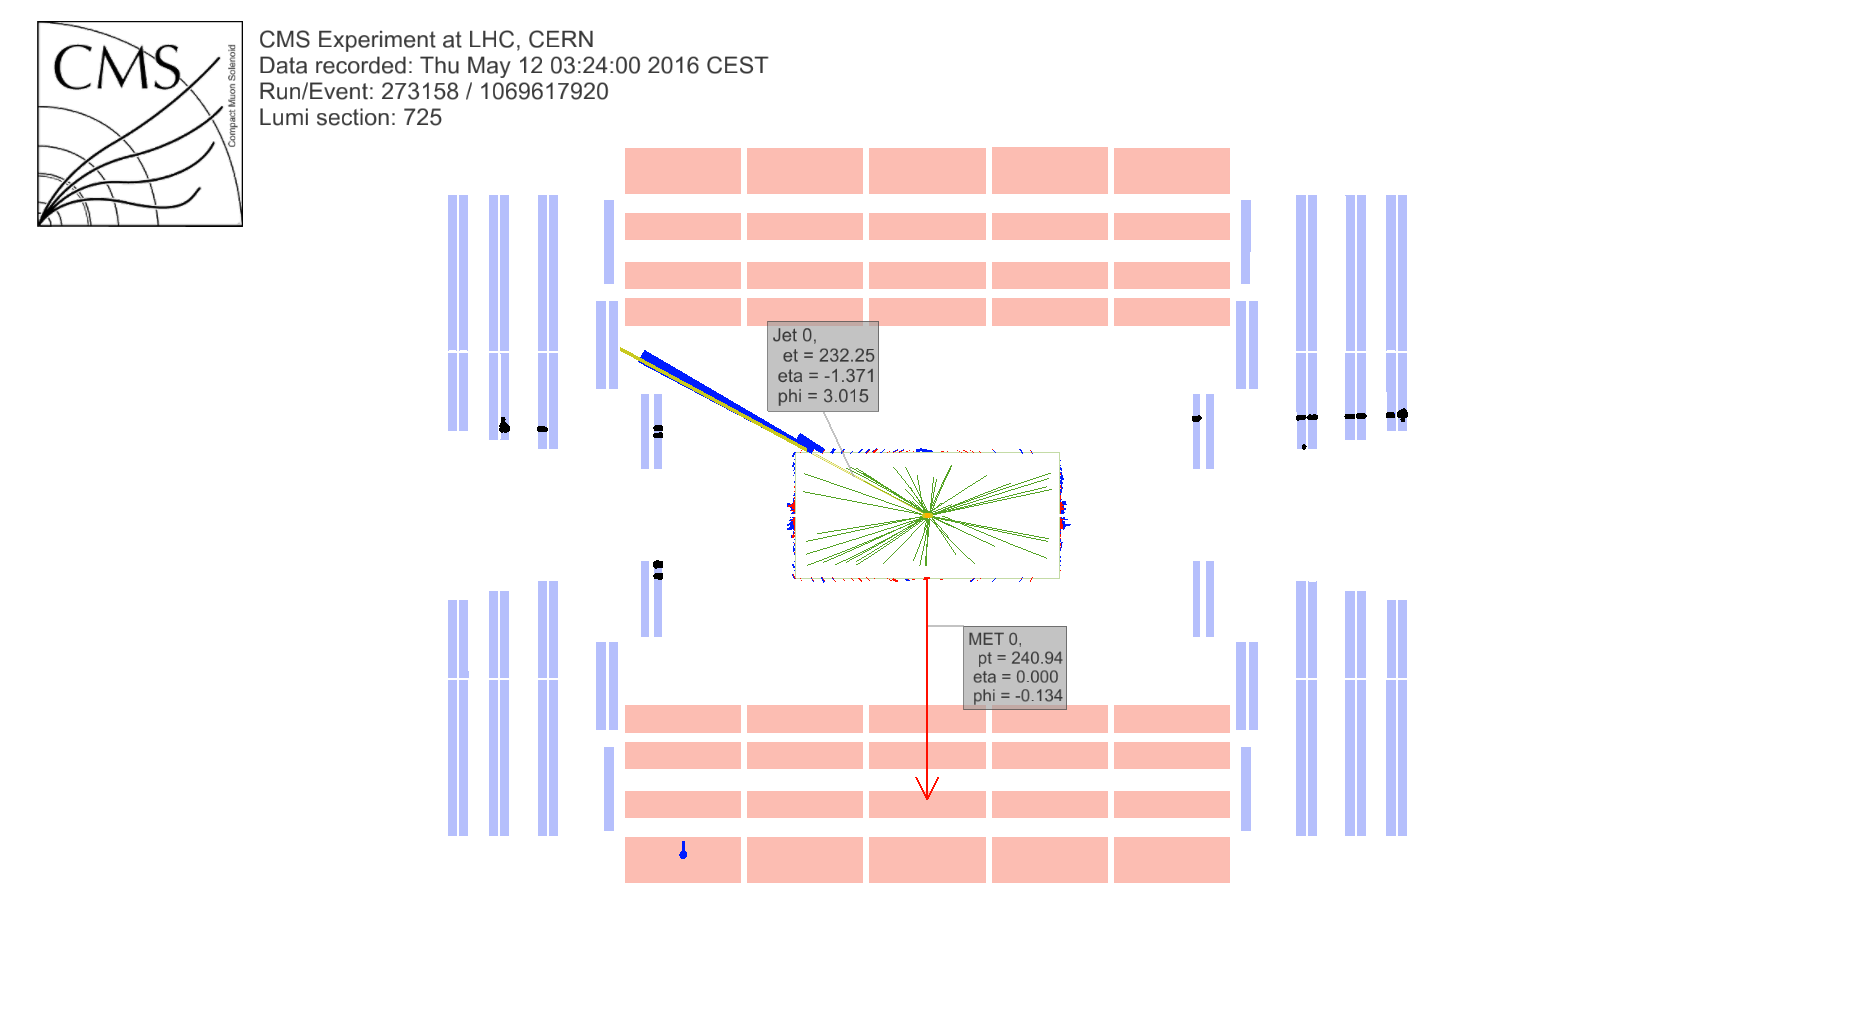
\includegraphics[width=1.\linewidth]{5_EventSelection/Figures/Figure_004}
	\caption{Event display of a beam halo event with collinear hits in the CSC (black), missing transverse energy of 250 \GeV\, and a jet of 232 \GeV. The hadronic deposit is spread in $\eta$, but narrow in $\phi$. Figure taken from~\cite{CMS-PAS-JME-16-004}. }
	\label{fig:beamhalo}
\end{figure}

Furthermore, there is anomalous high missing transverse energy coming from low quality muons that lead to high-\pt\ tracks, but are considered not good by the particle flow algorithm. These low quality tracks will be  mislabelled as charged hadrons and will therefore be used in the calculation of the missing transverse energy. By investigation the purity of the reconstructed tracks and the relative transverse momentum error of the muons, these events can be filtered out. 


% see https://indico.cern.ch/event/591506/contributions/2387636/attachments/1381281/2099935/2016_12_01_MET_Scanning_Report_PPD.pdf
% see https://indico.cern.ch/event/537458/contributions/2184619/attachments/1281045/1903148/met_scanner_report_may30.pdf
% see https://indico.cern.ch/event/534040/contributions/2178680/attachments/1280427/1901837/HCALnoise_JamboreeMeeting_27May2016.pdf
%see https://indico.cern.ch/event/518559/contributions/2132815/attachments/1264581/1871184/beamhalostatus.pdf
% see https://twiki.cern.ch/twiki/bin/viewauth/CMS/MissingETOptionalFiltersRun2


Supplementary to previous filters, only events with where the first primary vertex is a well reconstructed primary vertex are selected. The reconstructed primary vertex should have at least five degrees of freedom, the longitudinal distance from the beam spot is maximally 24 cm ($d_z < 24$ cm), and the transversal distance from the beam spot is maximally 2 cm ($d_{xy}<2$ cm). 
\subsection{Estimation of the trigger efficiency}
\label{sec:triggereff}
The trigger efficiency in data is estimated using a data sample collected using unprescaled \Etmis\ triggers. These allow events 
with a missing transverse energy higher then 110 \GeV (120 \GeV) and that the scalar sum of the transverse momenta of the reconstructed PF jets  $H_{\mathrm{T}}^{\mathrm{trig.}}$ is at least 300 \GeV\ (120 \GeV), or a calorimeter (PF) \Etmis\  higher than 200 \GeV (300 \GeV). For an HB-HE cleaned event the PF missing transverse energy threshold is lowered to 170 \GeV.  These trigger paths are summarised in \tab{tab:METtrig} and chosen to be completely uncorrelated with the lepton triggers given in \tab{tab:Trigger}. 
\begin{table}[htbp]
		\centering
		\caption{Unprescaled \Etmis\ HLT trigger paths for estimating the trigger efficiency. An \textit{or} of the triggers is used to select events.}
		\begin{tabular}{cc}
			\toprule
			Trigger path  & Requirement \\
			\midrule
	 HLT\_PFHT300\_PFMET110\_v* & PF \Etmis > 110 \GeV, PF $H_{\mathrm{T}}^{\mathrm{trig.}}$ > 300 \GeV \\
	 HLT\_MET200\_v* & calorimeter \Etmis > 200 \GeV  \\
	HLT\_PFMET300\_v* & PF \Etmis > 300 \GeV  \\
 HLT\_PFMET120\_PFHT120\_IDTight\_v* & PF \Etmis > 120 \GeV, PF $H_{\mathrm{T}}^{\mathrm{trig., tight WP}}$ > 120 \GeV \\
	 HLT\_PFMET170\_HBHECleaned\_v* & PF \Etmis > 170 \GeV,  cleaned for HB/HE anomalous signals \\
	 \bottomrule
	 \end{tabular}
 \label{tab:METtrig}
\end{table}

The trigger efficiency is studied on the main background, namely \WZ+jets, with all corrections applied. For this study, the events passing a three lepton cut and at least one jet are being used. The corresponding efficiencies are then calculated as
\begin{equation}
\epsilon_{data} = \frac{\textnormal{Nb. of events passing lepton and MET triggers}}{\textnormal{Nb. of events passing MET triggers}}
\end{equation}
\begin{equation}
\epsilon_{MC} = \frac{\textnormal{Nb. of events passing lepton triggers}}{\textnormal{Nb. of total events}}
\end{equation}
The resulting efficiencies and scale factors can be found in  \tab{tab:trigSFe}, where the scale factors are defined as 
\begin{equation}
SF = \frac{\epsilon_{data}}{\epsilon_{MC}}.
\end{equation} 
More detailed scale factors and efficiencies can be found in \App{app:TriggerSF}.
\begin{table}[htbp]
	\centering
	\caption{Trigger scale factors for each channel, after three lepton + jets cut, in the Z mass window. by counting number of events.}
	\begin{tabular}{ccccc}
		\toprule 
		all & \mumumu & \eee & \eemu & \emumu \\ 
		\midrule 
		1.0000 & 1.0000 & 0.9541 & 1.0006  & 1.0004\% \\ 
		\bottomrule
	\end{tabular} 
	\label{tab:trigSFe}
\end{table}

The trigger efficiencies are also measured in function of the \pt\ of the leptons for which the distributions can be found in \App{app:TriggerSF}. The resulting scale factors in can be found in Figure \fig{image:FigurestriggerIntext}.
\begin{figure}[htbp]
	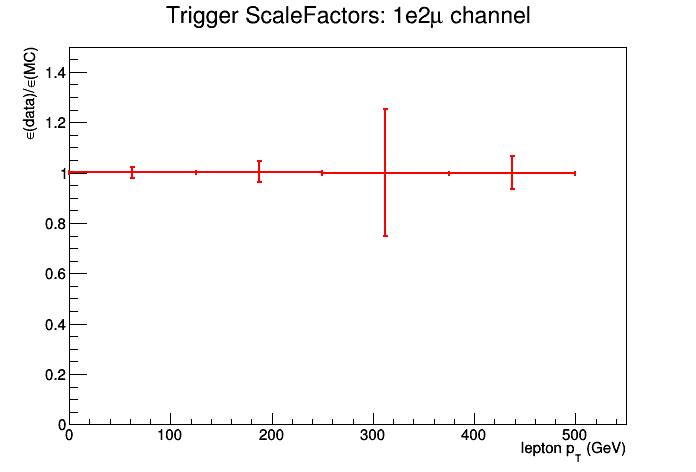
\includegraphics[width=0.48\textwidth]{Appendix/Figures/trigger/Intext/SF_trigger_1e2muhistPt.png}
	%		\label{image:SF_trigger_1e2muhistPt.png}
	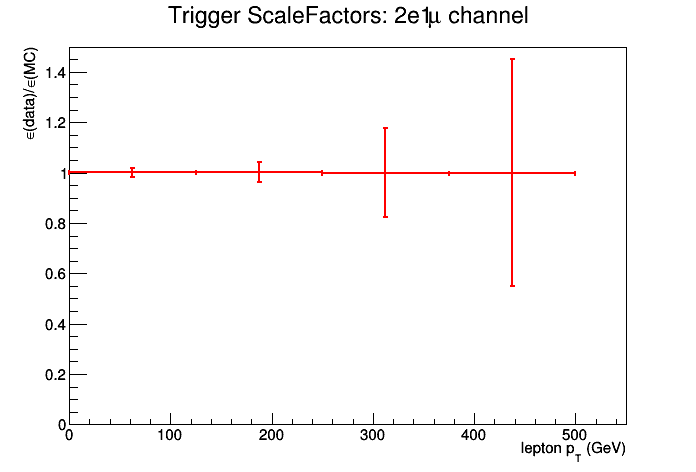
\includegraphics[width=0.48\textwidth]{Appendix/Figures/trigger/Intext/SF_trigger_2e1muhistPt.png}
	%		\label{image:SF_trigger_2e1muhistPt.png}
	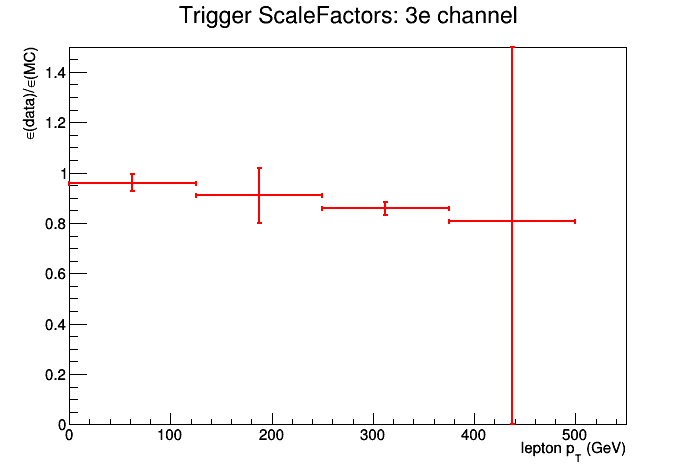
\includegraphics[width=0.48\textwidth]{Appendix/Figures/trigger/Intext/SF_trigger_3ehistPt.png}
	%		\label{image:SF_trigger_3ehistPt.png}
	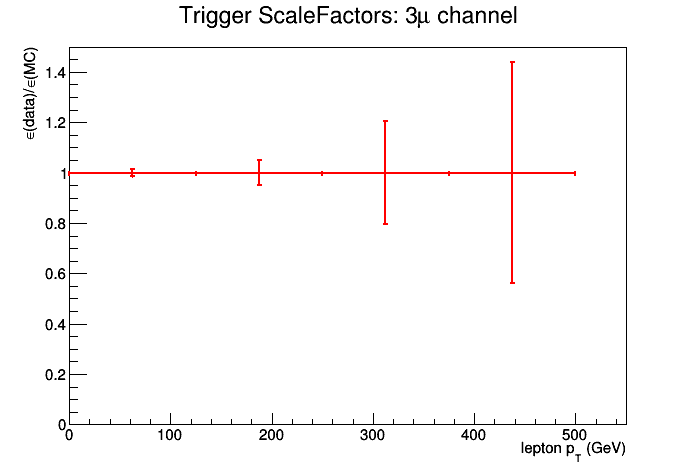
\includegraphics[width=0.48\textwidth]{Appendix/Figures/trigger/Intext/SF_trigger_3muhistPt.png}
	%		\label{image:SF_trigger_3muhistPt.png}
	
	\caption{The trigger scale factors measured as a function of lepton \pt, using the dataset collected by \Etmis\ triggers and \WZ\ simulation, after a 3 lepton and jets selection, in the Z mass window. All corrections to simulation are applied. Left, upper: \emumu\ channel. Right, upper: \eemu\ channel. Left, lower: \eee\ channel. Right, lower: \mumumu\ channel}
	\label{image:FigurestriggerIntext}
\end{figure}
The trigger efficiencies are measured to be nearly 100\% for both simulation and data. The results are dominated by statistics and assigning a large uncertainty to the trigger efficiency based on the dataset collected by \Etmis\ triggers would be over conservative. A one percent uncertainty on the trigger selection for the \eemu\ and \mumumu\ final states, and 5\% for the \eee\ and \emumu\ final states is assigned instead. No scale factors will be applied on simulation as they are close to unity. Control plots are made in the dilepton region to validate all corrections applied to simulation and can be found in \App{app:controldilep} \todo{Make sure this is the case}.

\subsection{Corrections}
\label{sec:corrections}
Mismatches between data and simulation are corrected for via the use of scale factors. These are elaborately discussed in \Sec{sec:PhysicsObject}. In this section a short overview of the applied corrections is given and their effect on a dilepton selection is shown. 

\subsubsection*{Pileup reweighting}
In data, the number of interactions per bunch crossing (pileup) is calculated with a minimum bias cross section of 69.2 mb. The number of simulated pileup events is then reweighed to match the expected number of pileup events in data. Pileup reweighting manifests itself as an altered shape of the number of reconstructed primary vertices as can be seen in \fig{fig:nbvertices}.

\begin{figure}[htbp]
	\centering	
	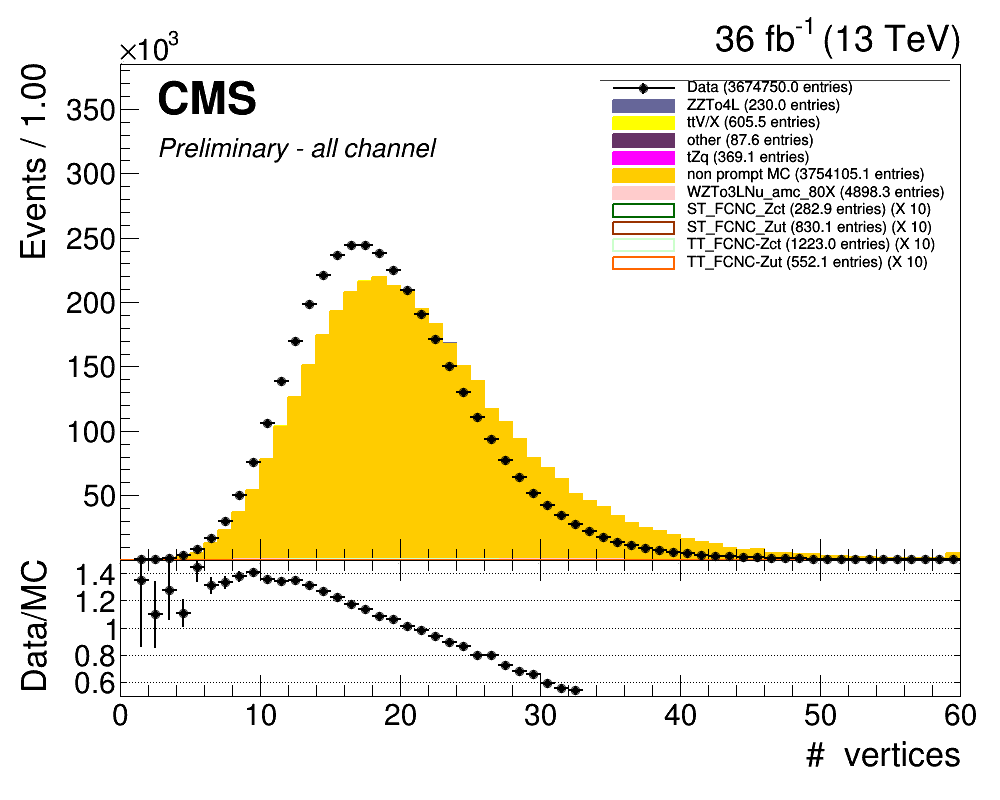
\includegraphics[width=0.45\textwidth]{5_Eventselection/Figures/Reweighing/pileup/2lepcontrol_afterAtLeast1Jet_afterZWindow_NbOfVertices_all_Stack_before}
	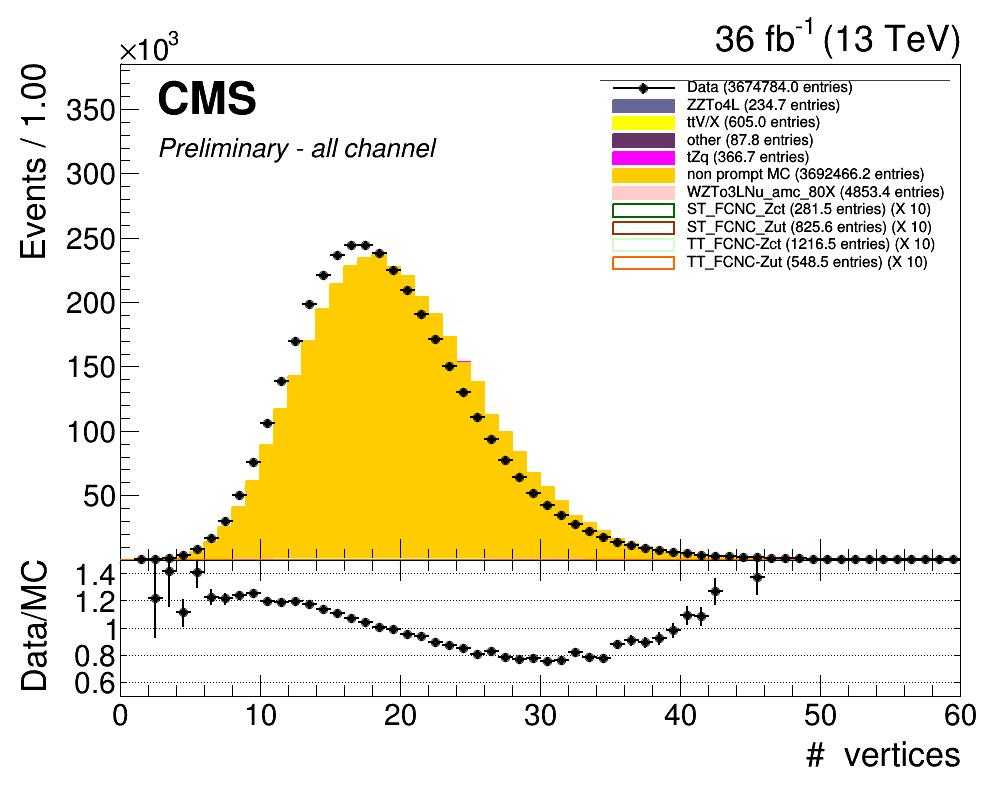
\includegraphics[width=0.45\textwidth]{5_Eventselection/Figures/Reweighing/pileup/2lepcontrol_afterAtLeast1Jet_afterZWindow_NbOfVertices_all_Stack}
	\caption{The number of primary vertices before (left) and after (right) pileup reweighting. After a dilepton plus jets selection, in the \PZ\ mass window.}
	\label{fig:nbvertices}
\end{figure}

Note that \fig{fig:nbvertices} indicates that even after pileup reweighting, the primary vertex multiplicity is not well described by simulation. This is a known effect, and using  a minimum bias cross section with a slightly lower value is found to better describe the data. However, the b tagging scale factors are only provided for the nominal inelastic cross section, and thus this value is used.


\subsubsection*{Lepton scale factors}
The efficiency to select leptons is different in simulation ($\epsilon_{\mathrm{MC}}$) compared to the data ($\epsilon_{\mathrm{data}}$). This is corrected for by applying lepton scale factors (SF) to the simulation that are defined as
\begin{equation}
SF = \frac{\epsilon_{\mathrm{data}}}{\epsilon_{\mathrm{MC}}}. 
\end{equation}
These scale factors are measured for the identification, isolation, tracking and trigger efficiencies of the objects as a function of \pt\ and $\eta$ (see \Sec{sec:MuonID} and \Sec{sec:ElectronID}). Multiplying these scale factors for each lepton provides an overall efficiency:
\begin{equation}
SF^{\mu}_{\mathrm{global}} = \prod \limits_{\mathrm{i}}^{\# \mu}  SF^{\mu}_{\mathrm{ID}}(\pt,\eta) \: SF^{\mu}_{\mathrm{Iso.}}(\pt,\eta)\: SF^{\mu}_{\mathrm{Trig.}}(\pt,\eta) \:SF^{\mu}_{track}(\pt,\eta),
\end{equation}
\begin{equation}
SF^{\mathrm{e}}_{\mathrm{global}} = \prod \limits_{\mathrm{i}}^{\# e}  SF^{\mathrm{e}}_{\mathrm{ID}}(\pt,\eta)\: SF^{\mathrm{e}}_{\mathrm{Iso.}}(\pt,\eta) \: SF^{\mathrm{e}}_{\mathrm{Trig.}}(\pt,\eta) \: SF^{\mathrm{e}}_{track}(\pt,\eta) .
\end{equation}
The effect of the scale factors can be found in \fig{fig:elSF} for the electron scaling and \fig{fig:muSF} for the muons. The trigger efficiencies are estimated in Section \ref{sec:triggereff}.

\begin{figure}[htbp]
	\centering
	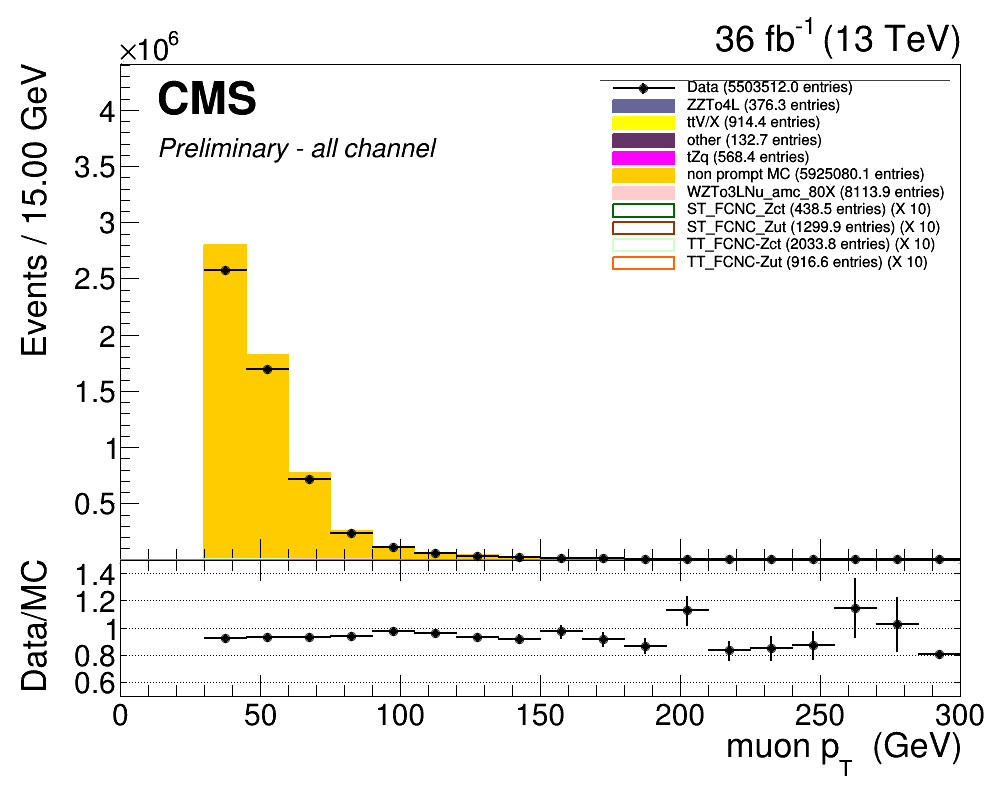
\includegraphics[width=0.45\textwidth]{5_Eventselection/Figures/Reweighing/muon/2lepcontrol_afterAtLeast1Jet_afterZWindow_MuPt_all_Stack_before}
	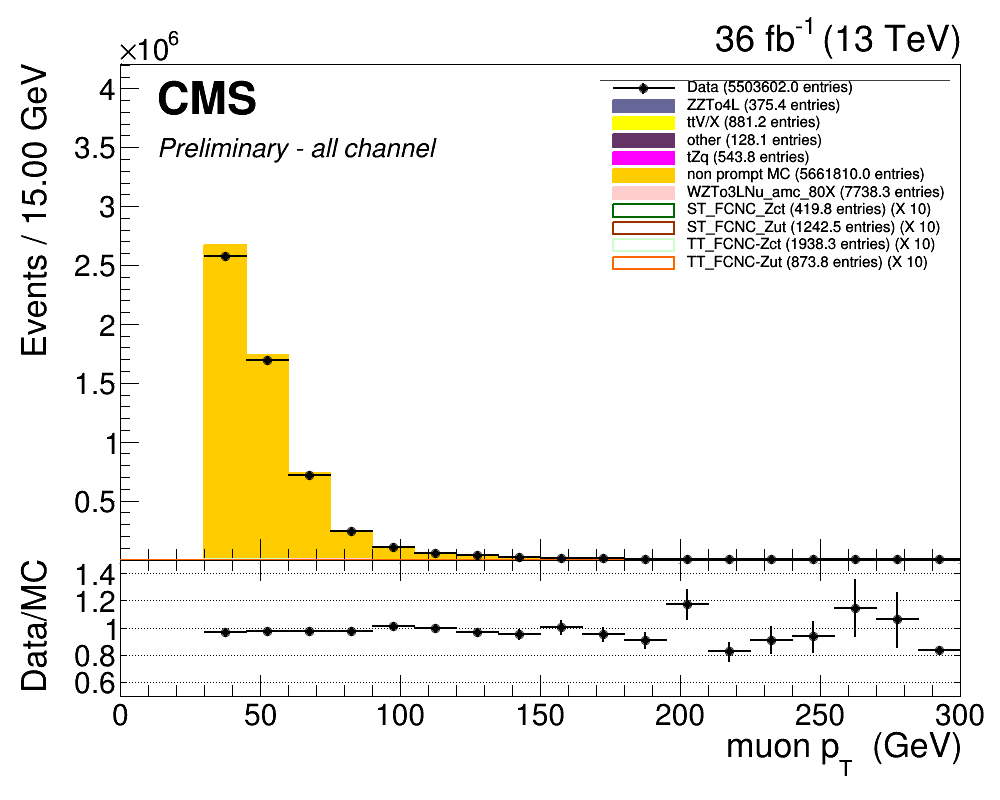
\includegraphics[width=0.45\textwidth]{5_Eventselection/Figures/Reweighing/muon/2lepcontrol_afterAtLeast1Jet_afterZWindow_MuPt_all_Stack_after}
	\caption{The \pt\ of the muons before (left) and after (right) muon scale factors. After a dilepton plus jets selection, in the \PZ\ mass window. Both after the Rochester correction.}
	\label{fig:muSF}
\end{figure}
\begin{figure}[htbp]
	\centering
	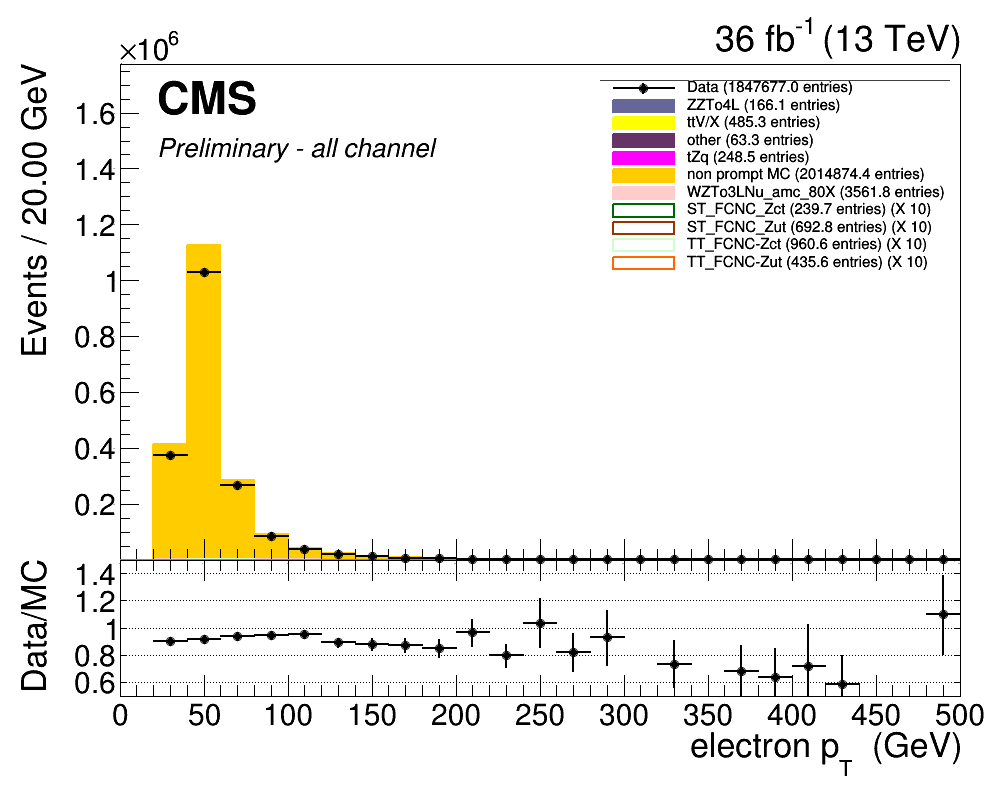
\includegraphics[width=0.45\textwidth]{5_Eventselection/Figures/Reweighing/electron/2lepcontrol_afterAtLeast1Jet_afterZWindow_ElPt_all_Stack_before}
	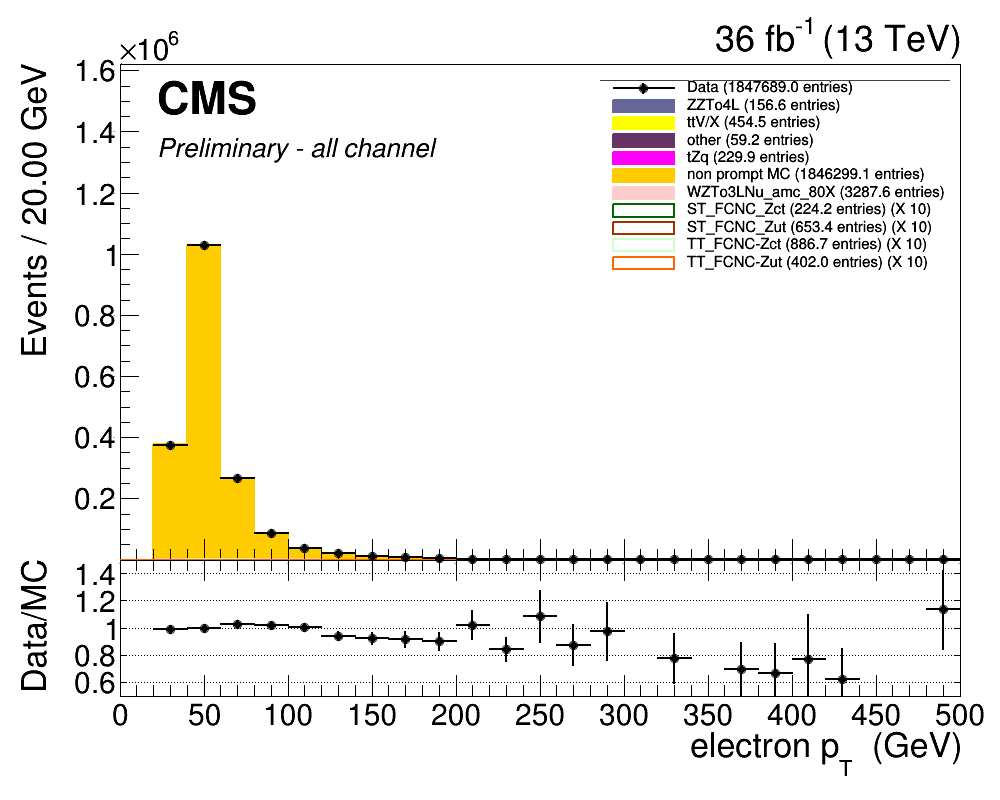
\includegraphics[width=0.45\textwidth]{5_Eventselection/Figures/Reweighing/electron/2lepcontrol_afterAtLeast1Jet_afterZWindow_ElPt_all_Stack_after}
	\caption{The \pt\ of the electrons before (left) and after (right) electron scale factors. After a dilepton plus jets selection, in the \PZ\ mass window. Both after energy scale corrections and smearing.}
	\label{fig:elSF}
\end{figure}

Additionally, corrections are made for the energy resolution of the leptons. For the electrons, energy smearing and regression is applied \cite{smearing}. The energy regression uses the detector information to correct the electron energy in order to have the best energy resolution by correcting local energy containment, material effects, etc.. The energy scale and smearing is done in order to bring the data energy scale to simulation level. It smears the simulation energies to have identical energy resolution in simulation and data. For the muons, the \pt\ is corrected using the Rochester method \cite{roch,roch2}. This correction removes the bias of the muon \pt\ from any detector misalignment or any possible error of the magnetic field.
The effect of the Rochester correction can be found in \fig{fig:roch}.

\begin{figure}[htbp]
	\centering	
	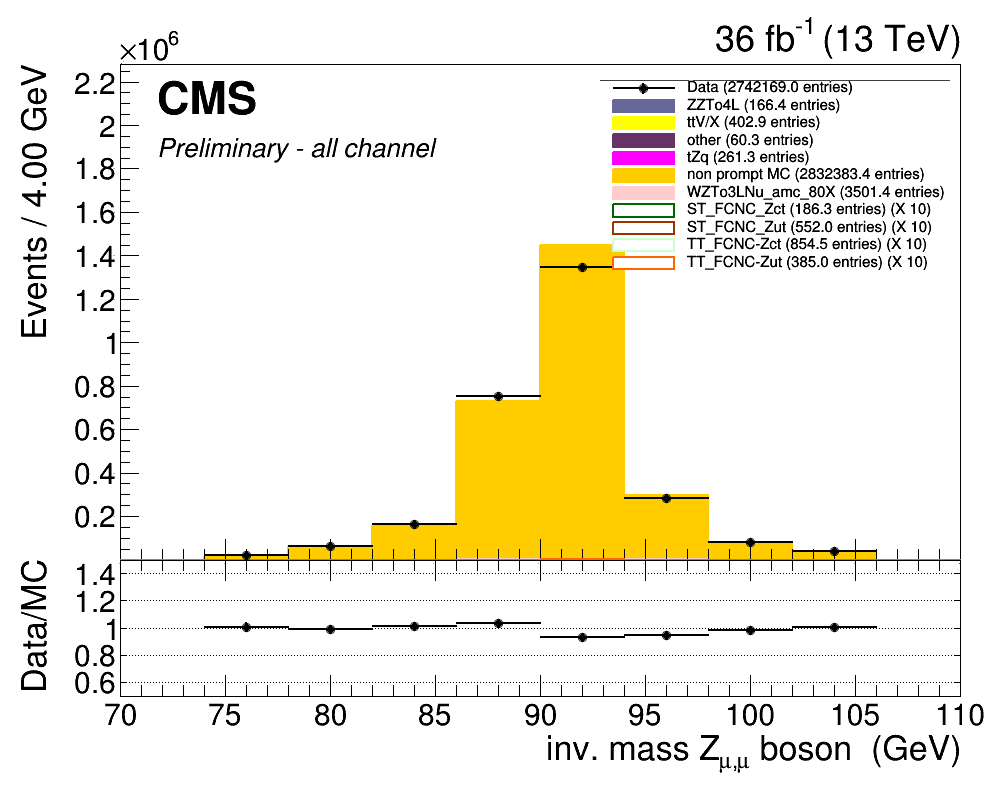
\includegraphics[width=0.45\textwidth]{5_Eventselection/Figures/Reweighing/rochester/2lepcontrol_afterAtLeast1Jet_afterZWindow_ZbosonMassMu_all_Stack_before}
	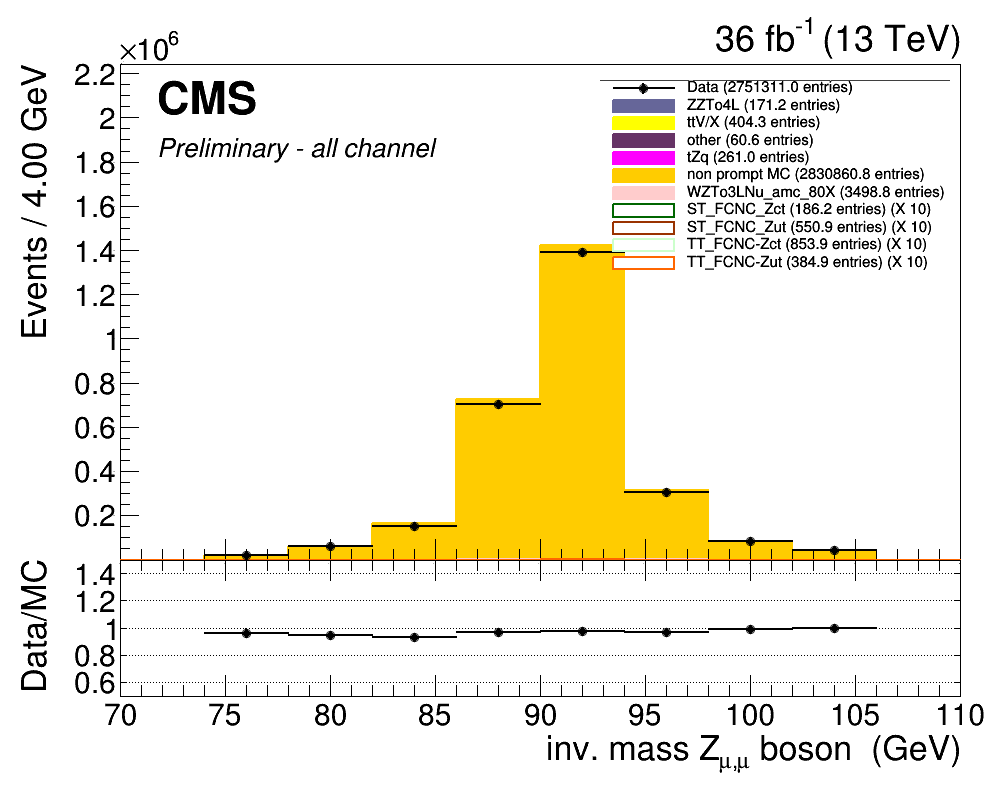
\includegraphics[width=0.45\textwidth]{5_Eventselection/Figures/Reweighing/rochester/2lepcontrol_afterAtLeast1Jet_afterZWindow_ZbosonMassMu_all_Stack_after}
	
	\caption{The mass of the \PZ\ boson consisting of the muons before (left) and after (right) the rochester correction. After a dilepton plus jets selection, in the \PZ\ mass window.}
	\label{fig:roch}
\end{figure}
\newpage
\subsubsection*{CSVv2 shape correction}
In order to make the shape of the CSVv2 b-tagging discriminant in simulation agree with data,  jet-by-jet based scale factors are applied. These scale factors are a function of the \pt, $\eta$ and CSVv2 value of the jet as discussed in \Sec{sec:BJetID}.  The effect of these scale factors can be found in \fig{fig:bSF}.


\begin{figure}[htbp]
	\centering
	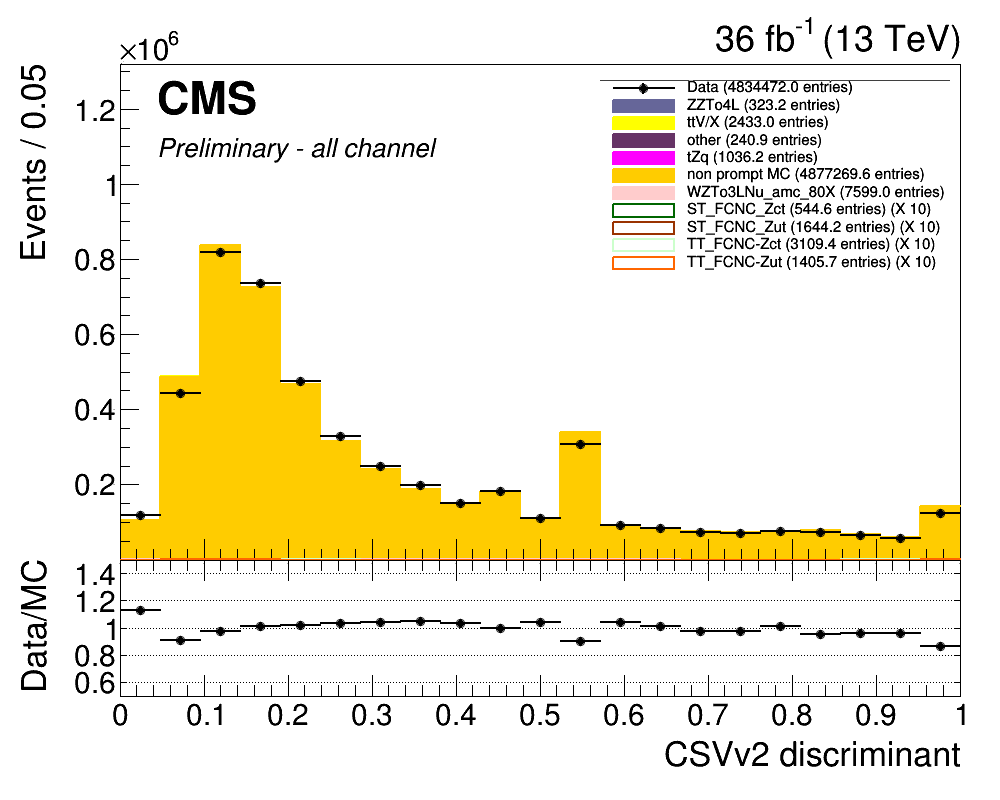
\includegraphics[width=0.45\textwidth]{5_Eventselection/Figures/Reweighing/bdis/2lepcontrol_afterAtLeast1Jet_afterZWindow_bdisc_all_Stack_before}
	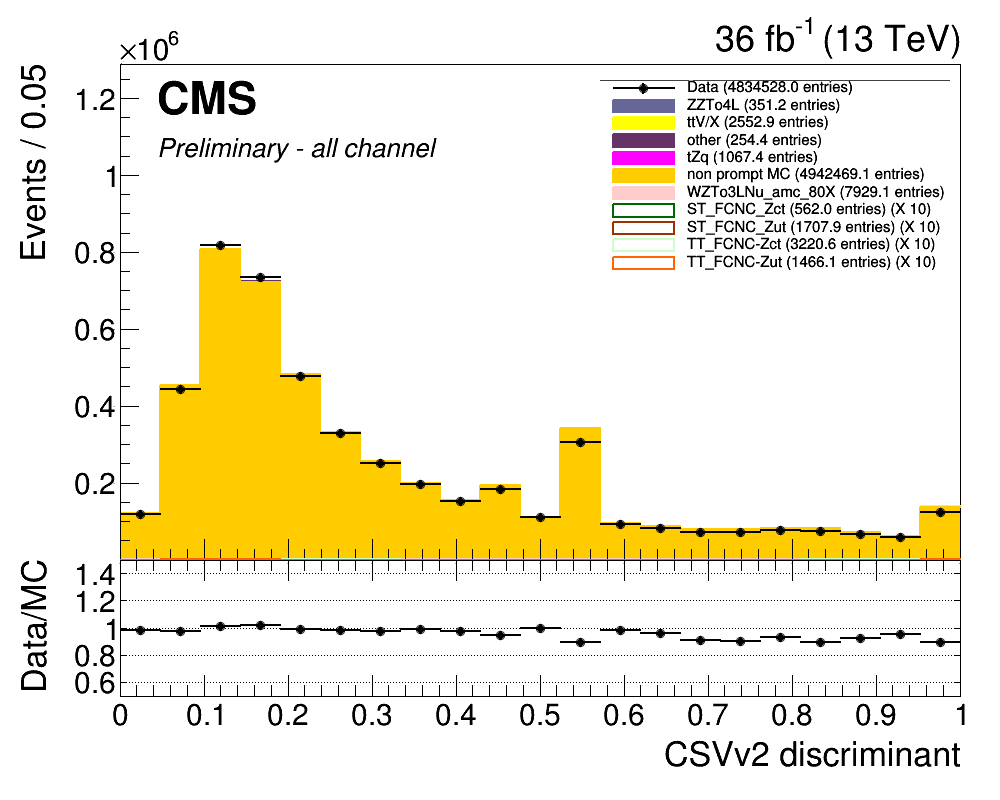
\includegraphics[width=0.45\textwidth]{5_Eventselection/Figures/Reweighing/bdis/2lepcontrol_afterAtLeast1Jet_afterZWindow_bdisc_all_Stack_after}	
	\caption{The CSVv2 discriminant of the jets before (left) and after (right) b-tag scale factors. After a dilepton plus jets selection, in the \PZ\ mass window.}
	\label{fig:bSF}
\end{figure}

\subsubsection*{Jet energy}
\label{sec:jer}
The jet energy in data and simulation is corrected by the measured energy response of the detector. This provides $p_T$- and $\eta$ dependent scale factors and are directly taken from the frontier condition database as discussed in \Sec{sec:JetID}. 
%Additionally, the jet \pt\ resolution is corrected by the scaling method described in \cite{jetsmear}, where the jet \pt\ is rescaled by
%\begin{equation}
%c_{\mathrm{JER}} = 1 + (s_{\mathrm{JER}}-1)\frac{\pt -\pt^{ptcl}}{\pt}.
%\end{equation}
%With \pt\ the reconstructed transverse momentum, \pt$^{ptcl}$ the transverse momentum of the corresponding jet clustered from generator level particles, and $s_{\mathrm{JER}}$ the resolution scale factor. The resolution scale factor is measured in $\eta$ bins and given in Table \ref{tab:JER}. 
The effect of the jet energy corrections can be found in \fig{fig:jesSF} and \fig{fig:jerSF}. \todo{Fix jer plot}

\begin{figure}[htbp]
	\centering
	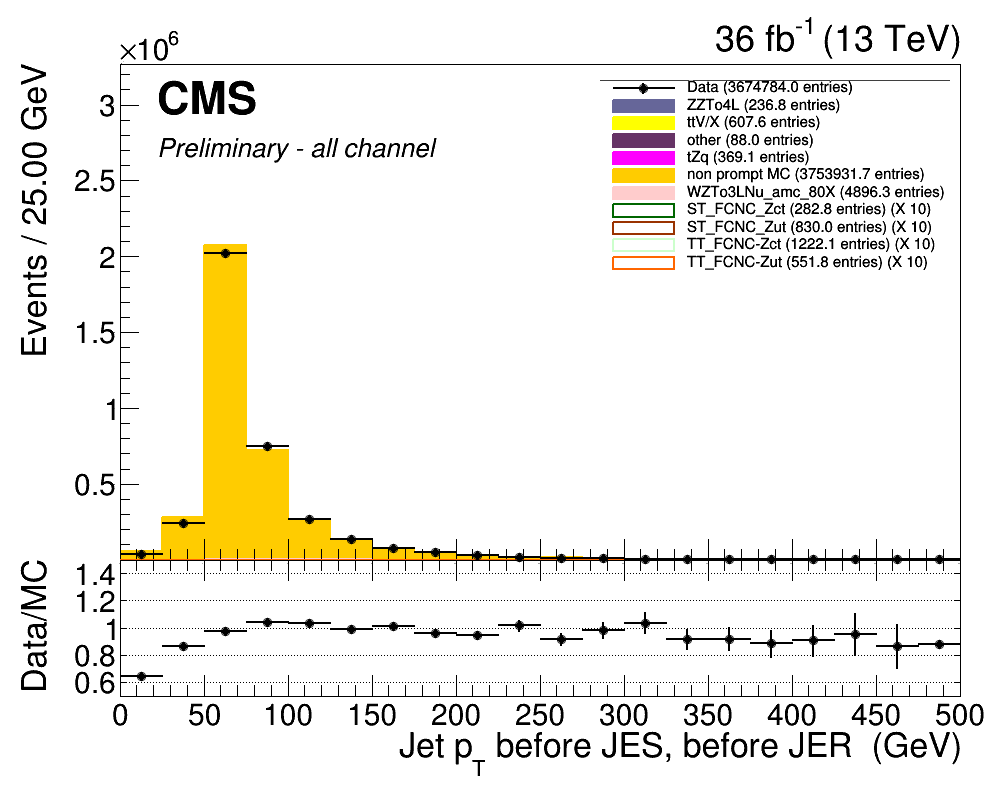
\includegraphics[width=0.45\textwidth]{5_Eventselection/Figures/Reweighing/JEC/2lepcontrol_afterAtLeast1Jet_afterZWindow_JetPt_bfJES_all_Stack}
	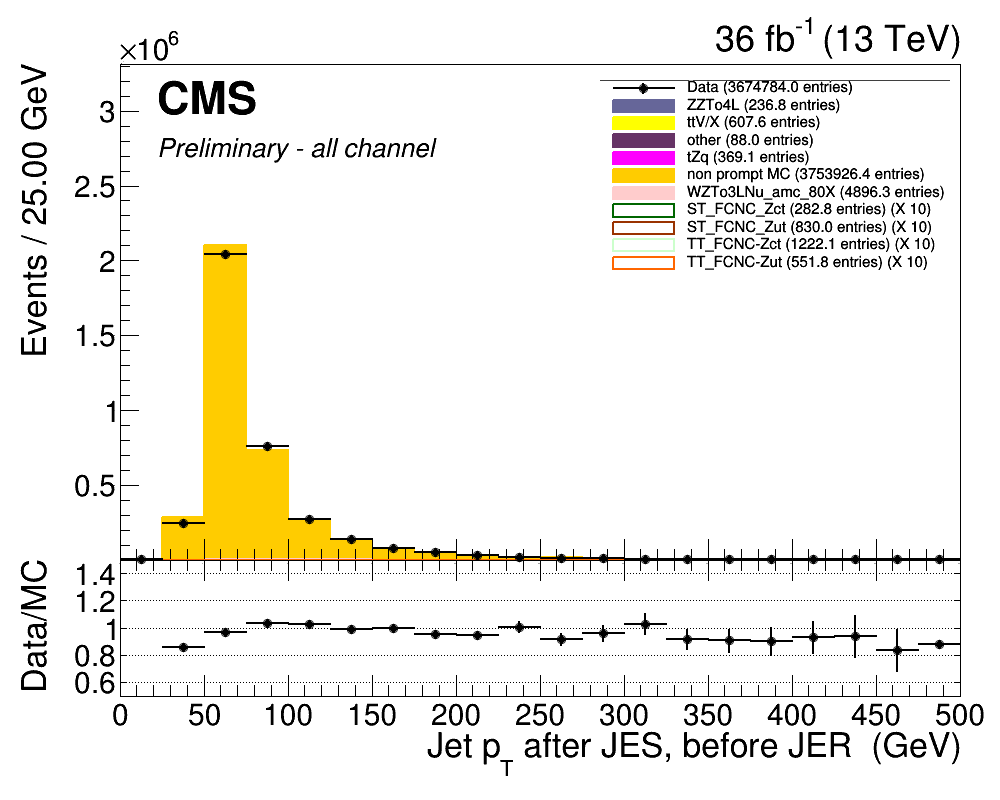
\includegraphics[width=0.45\textwidth]{5_Eventselection/Figures/Reweighing/JEC/2lepcontrol_afterAtLeast1Jet_afterZWindow_JetPt_afJES_all_Stack}
	\caption{The \pt\ of the jets before (left) and after (right) jet energy scale corrections. After a dilepton plus jets selection, in the \PZ\ mass window.}
	\label{fig:jesSF}
\end{figure}

\begin{figure}[htbp]
	\centering
	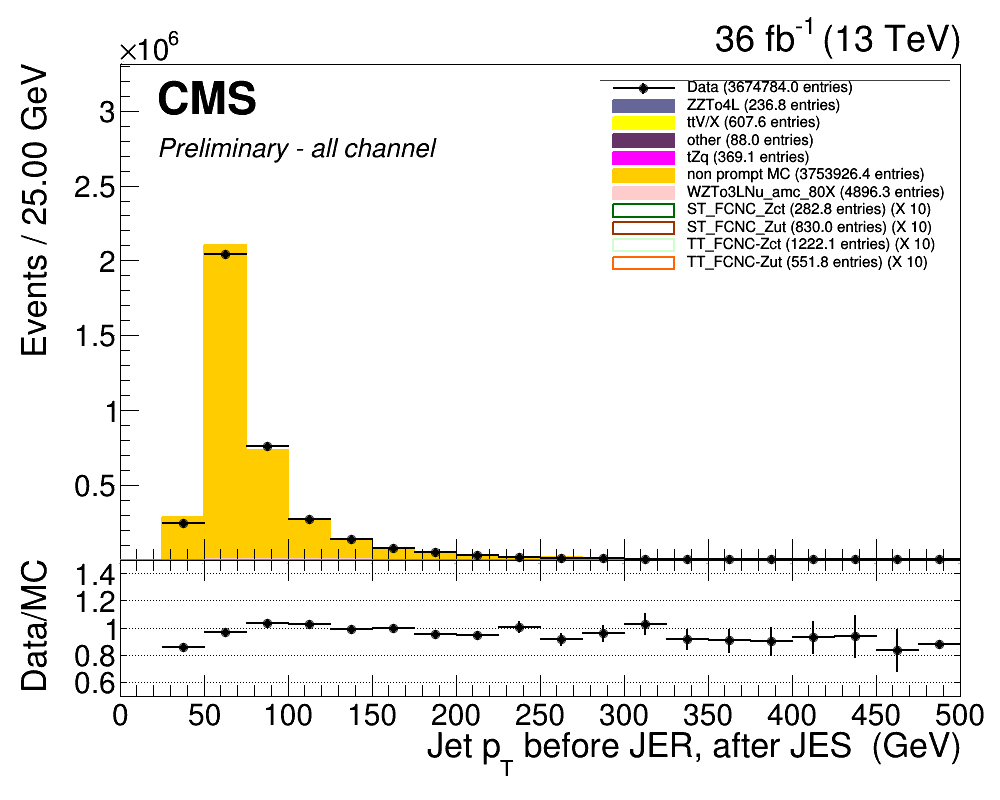
\includegraphics[width=0.45\textwidth]{5_Eventselection/Figures/Reweighing/JER/2lepcontrol_afterAtLeast1Jet_afterZWindow_JetPt_bfJER_all_Stack}
	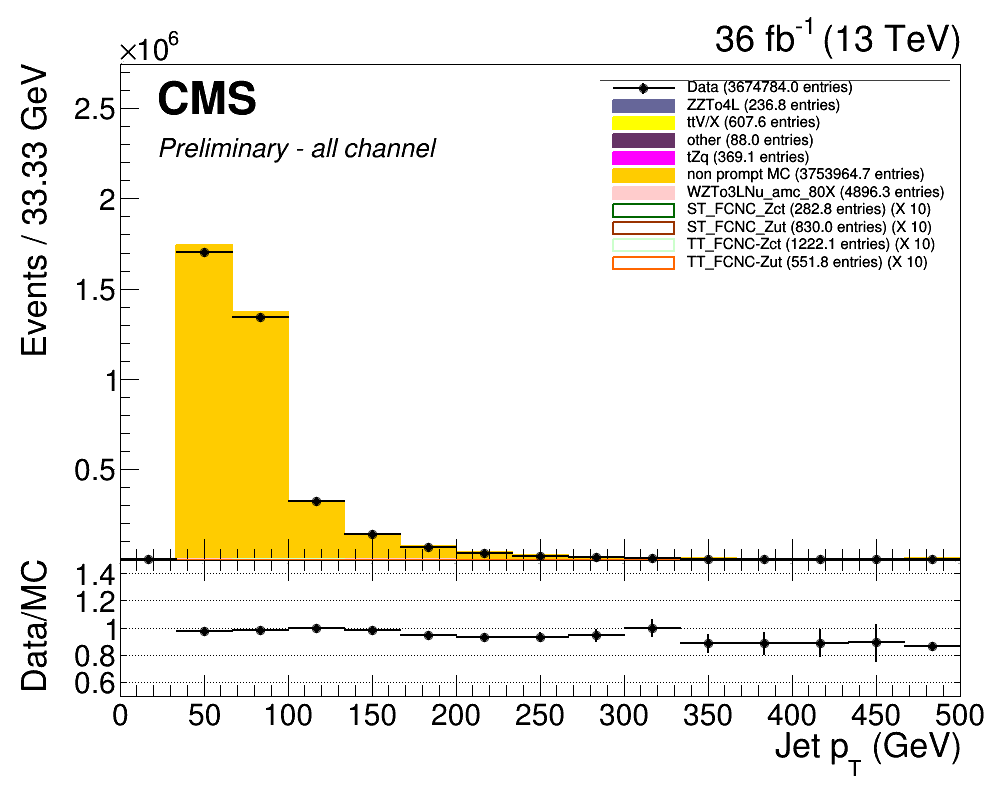
\includegraphics[width=0.45\textwidth]{5_Eventselection/Figures/Reweighing/JER/2lepcontrol_afterAtLeast1Jet_afterZWindow_JetPt_afJER_all_Stack}
	\caption{The \pt\ of the jets before (left) and after (right) jet energy resolution smearing. After a dilepton plus jets selection, in the \PZ\ mass window.}
	\label{fig:jerSF}
\end{figure}


\subsubsection*{Missing transverse energy}
The energy scale and resolution corrections applied to the jets are propagated back to the  missing transverse energy (smeared Type I correction) as discussed in \Sec{sec:MET}. This rebalances the transverse net momentum of the event and improves the missing transverse energy resolution itself.

\subsection{Reconstruction of kinematic variables}
The variables used for  the training are related to the reconstructed leptons, jets, \PZ\ boson and top quark candidates. The \PZ\ boson is reconstructed as the sum of the four vectors of the two same flavour leptons of opposite sign giving the closest value to the \PZ\ mass. The third remaining lepton is assigned as the lepton coming from the \PW\ boson decay.
The reconstruction of the \SM\ top quark candidate is more difficult and done by summing the third lepton, the \SM\ b-jet and the neutrino (\Etmiss). The \SM\ b jet is assigned to the jet with the highest CSVv2 discriminant. The longitudinal momentum of the neutrino is calculated by putting a constraint on the lepton+neutrino system with the \PW\ mass. In case two solutions are found for the $p_z^{\nu}$ component, the one that gives the reconstructed mass (lepton + neutrino + b jet) to  the known top quark mass is used. 
The FCNC top quark is reconstructed by summing the reconstructed Z boson and the jet giving the mass closest to the top mass, from the jet collection from which the \SM\ b jet is removed. 

The reconstructed objects are validated using simulation by matching the reconstructed objects to their generated counterpart by minimizing $\Delta R$. The efficiencies derived for the simulated signal samples and the \SM\ \tZq\ background process can be found in \tab{tab:matching} and \tab{tab:matching2}. 

\begin{table}[htbp]
	\centering
	\caption{Efficiencies of assigning the correct leptons in the analysis.}
	\begin{tabular}{cccc}
		\toprule 
		& FCNC \tZq  & FCNC \tZ & \SM\ \tZq \\ 
		\midrule
		\PW\ lepton & 99\% & 98\% & 97\% \\ 
	
		leptons from the \PZ\ boson  & 99\% & 98\% & 97\% \\ 
		 
		all leptons in the decay & 99\% & 98\% & 97\% \\ 
		\bottomrule
	\end{tabular} 
	\label{tab:matching}
\end{table}


\begin{table}[htbp]
	\centering
	\caption{Efficiencies of assigning the correct jets in the analysis.}
	\begin{tabular}{cccc}
		\toprule
		& FCNC \tZq  & FCNC \tZ & SM \tZq \\ 
		\midrule
		\SM\ \Pbottom\ jet & 99\% & 98\% & 80\%\\ 
		\Pcharm\ jet  & 71\% & N/A & 50\% \\  
		\Pup\ jet  & 83\% & N/A & 54\% \\ 
		\bottomrule
	\end{tabular} 
	\label{tab:matching2}
\end{table}


\section{Analysis Strategy}
\label{sec:selection}

The analysis strategy uses five statistically independent regions to extract limits using a likelihood fit of various observables. Two signal regions, the \tZ\ (\STSR) and \tZq\ (\TTSR) signal regions, are constructed using the jet multiplicity,  focussed on each signal signature (see Tab. \ref{tab:Regions}).  In order to constrain the rate of \WZ+jet events as well as that of \NPL\ backgrounds, three control regions are defined. The \WZ\ control region (\WZCR) focusses on \NPL s originating from \DY\ and simultaneously constrains the \WZ+jets background rate. The \NPL\ backgrounds coming from a \ttbar\ process are constrained by two control regions, \TTCR\ and \STCR, one for each signal region (\TTSR\ and \STSR).  In the \STSR\ and \TTSR\, multivariate discriminants based on Boosted Decision Trees (BDT) (see \Sec{sec:BDT}) are used to respectively discriminate \FCNC\ \tZ\ and \FCNC\ \tZq\ from backgrounds. In the \WZCR\ a  discriminating variable between the two backgrounds, \WZ+jets and \NPL s, is used. In \TTCR\ and \STCR\, the dominating process is the \ttbar\ process, and its rate is estimated by subtracting all other background predictions from data. A simultaneous global fit using the \texttt{Higgs Combined Tool} (\Sec{sec:Stat}) is performed taking into account each region (\STSR, \TTSR, \WZCR, \TTCR\ and \STCR) for the four different leptonic channels. 


\section{Data driven \NPL\ background simulation}
\label{sec:NPL}
 One of the most important background consist of events with not prompt leptons. These are mostly instrumental background and are therefore very difficult to model. The \NPL\ background is estimated from data for both its shape and its normalisation. 

The \NPL\ background originates from hadronic objects wrongly reconstructed as leptons, real leptons coming from the semi-leptonic decay of a \Pbottom\ or \Pcharm\ hadron, or real leptons coming from the conversion of photons that pass the identification and isolation requirements. The dominant source of these \NPL s depend on the flavour of the lepton and therefore the events with a not prompt muon (\NPM) are treated differently than those with a not prompt electron (\NPE). For muons, the dominant source is the semi-leptonic decay of heavy flavour hadrons, while for electrons, the dominant sources are hadrons and photon conversions. 

The backgrounds causing \NPL\ contributions are mostly \DY (Drell--Yan) and \ttbar+jets dilepton processes, and in a smaller amount \WW\ processes. All of these backgrounds contain two real leptons and one \NPL. Due to the fact that the probability for a lepton to be a \NPL\ is small, backgrounds containing two or more \NPL\ s are neglected in thus search. The assumption is made that for \DY\ the two leptons compatible with a \PZ\ boson decay are the real leptons, and the additional lepton is coming from a \NPL\ source, while for \ttbar+jets the \NPL\ is associated to the Z boson. This has been validated using Monte Carlo simulation.

The \NPL\ sample is constructed from data by requiring exactly three leptons, from which two are considered real, isolated leptons and the third lepton is identified as a \NPL. This \NPL\ is created by loosening its identification and inverting its isolation criteria. The full requirements on the not prompt leptons are given in  \tab{tab:nonpromptel} and \tab{tab:nonpromptmu}. For \NPE s, a large fraction is coming from misidentified photons. These are removed by applying a tighter cut on the $1/E-1/p$ variable, and by limiting the isolation values to be smaller than one. 
\begin{table}[htbp]
	\centering
	
	\caption{Non prompt electron requirements used in this analysis. The requirements are set in the barrel ($|\eta_{supercluster}| \leq 1.479$)
		and the end caps ($|\eta_{supercluster}| > 1.479$). }
	\begin{tabular}{ccc}
		\toprule
	 Properties	& \multicolumn{1}{c|}{$|\eta_{supercluster}| \leq 1.479$ } & \multicolumn{1}{c}{$|\eta_{supercluster}| > 1.479$ } \\
		\midrule
		$\sigma_{\eta \eta}$ & $<$ 0.011 & $<$ 0.0314 \\ 
		
		$|\Delta\eta_{\mathrm{in}}|$ & $<$ 0.00477& $<$ 0.00868\\ 
		
		$|\Delta\phi_{\mathrm{in}}|$ & $<$ 0.222 &  $<$ 0.212 \\ 
		 
		H/E & $<$ 0.298& $<$ 0.101 \\ 
		
		relative isolation & $\geq$ 0.0588 \&\& $<$ 1 &  $\geq$ 0.0571 \&\& $<$ 1\\ 
	
		$|1/E-1/p|$ & $<$ 0.0129 \GeVinv & $<$ 0.0129 \GeVinv \\ 
		
		expected missing inner hits & $\leq $ 1 &  $\leq $ 1\\ 
	
		pass conversion veto & Y & Y \\ 
	
		\pt &$>$ 35 \GeV & $>$ 35 \GeV \\
		\bottomrule
	\end{tabular} 
	\label{tab:nonpromptel}
\end{table}

\begin{table}[htbp]
	\centering
	\caption{Non prompt muon requirements used in the analysis. }
	
	\begin{tabular}{cc}
		\toprule
	 Properties	& modified Loose Muon WP \\ 
		\midrule 
		Global muon or Tracker Muon & Both  \\ 
		
		Particle Flow muon & Y  \\ 
		
		$\chi^2/ndof$ of global muon track fit & N/A \\  
		
		Nb. of hit muon chambers & N/A \\ 
		 
		Nb. of muon stations contained in the segment & N/A   \\ 
		
		Size of the transverse impact parameter  of the track wrt. PV & N/A  \\ 
		 
		Longitudinal distance wrt. PV & N/A \\ 
		
		Nb. of pixel hits & N/A \\ 
		
		Nb. of tracker layers with hits & N/A  \\ 
		
		Relative Isolation & $\geq$ 0.15 \\
		
		\pt &$>$ 30 \GeV  \\
		\bottomrule
	\end{tabular} 
	
	\label{tab:nonpromptmu}
\end{table}


\newpage
\section{Regions and channels}
\label{sec:regions}
The regions are defined as in Table \ref{tab:Regions} after a common selection of exactly three leptons containing one opposite sign, same flavour pair that is assigned to the \PZ\ boson, at least one jet and at the most three jets, the transverse mass of the \PW\ boson to be maximal 300 \GeV. %The cut on the transverse mass of the \PW\ boson is done to remove events that are passing the events cleaning elading to anomalous large missing transverse energy.
The transverse mass $\mtw$ is reconstructed using
\begin{equation}
\mtw = \sqrt{(\pt(l_{\W}) + \pt(\nu_{\W}) ) ^2 - (p_{\mathrm{x}}(l_{\W}) + p_{\mathrm{x}}(\nu_{\W}))^2  - (p_{\mathrm{y}}(l_{\W}) + p_{\mathrm{y}}(\nu_{\W}))^2    }
\end{equation}

\begin{table}[htbp]
	\centering
	\caption{The statistically independent regions used in the analysis.}
	\begin{tabular}{cccccc}
		\toprule
%		& \WZ  & \tZ  & \tZq  & \tZ  & \tZq\\ 
%		&  control region &  signal region & signal region &  control region & control region\\ 
		& \WZCR& \STSR  & \TTSR & \STCR & \TTCR \\ 
		\midrule
		Number of jets & $\geqslant 1$ & 1 & $\geqslant 2$  & 1 & $\geqslant 2$\\ 
		 
		Number of b jets & 0 & 1 & $\geqslant 1$  & 1 & $\geqslant 1$ \\ 
		
		$|\mZ^{\mathrm{reco}} - \mZ|< 7.5$ \GeV & Yes & Yes & Yes & No & No \\
		\hdashline
		$|\mZ^{\mathrm{reco}} - \mZ|< 30$ \GeV & Yes & Yes & Yes & Yes & Yes \\
			Number of leptons & 3 & 3 & 3  & 3 & 3\\
		\bottomrule 
	\end{tabular} 
	\label{tab:Regions}
\end{table}

Additional leptons with a looser identification are vetoed in order to reduce the contamination of backgrounds with four or more leptons in the final state, e.g. \ZZ, \ttZ, and \ttH. The most important backgrounds are the ones that contain three prompt leptons in the final state. These are mainly \WZ +jets, \ttZ\ and SM \tZq. For these backgrounds, the three lepton topology is identical to the \FCNC\ signal: two opposite sign leptons of the same flavour decaying from the \PZ\ boson, and a third additional, high \pt\ lepton coming from the \PW\ boson decay.

For the FCNC \tZ\ final state, one \Pbottom\ jet coming from the \SM\ top decay is expected. For the FCNC \tZq, an additional light jet is expected. In the \ttZ\ final state, two b jets are present in the final state. However, due to inefficiencies of the b-tagging algorithm, one of the two \Pbottom\ jets may be identified as a light quark jet, giving the same final state as the FCNC \tZq\ final state. For the \WZ+jets final states, one of the b jets produced by gluon splitting can be b-tagged or light flavour jets coming from the \WZ+jets production can be mis-tagged as b jets. The SM \tZq\ final state expects the same signal as FCNC \tZq.

The \NPL\  events give a significant background contribution. This background is coming mainly from \DY\ and \ttbar+jets processes (in a less significant way, also \WW\ and \tWZ\ contributes), which have very high cross sections and causes a large number of \NPL\  background events compared to signal.

In order to reduce the large uncertainties in backgrounds, five independent regions are used as defined in Table  \ref{tab:Regions}. In \fig{fig:regions}, the strategy and usage of each region is illustrated.
\begin{figure}
	\centering
	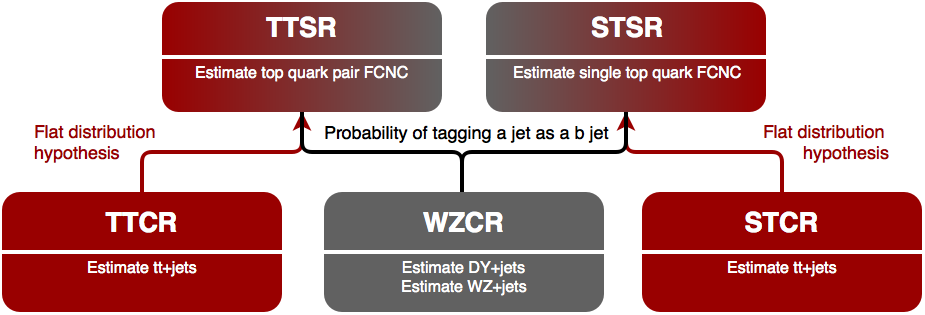
\includegraphics[width=1.\linewidth]{5_EventSelection/Figures/regions}
	\caption{The strategy used for this search. The \WZCR\ region is used to estimate the \WZ+jets background process as well as the \NPL\ background coming from the \DY\ process. The \TTCR\ and \STCR\ regions are used to estimate the contributions of the \NPL\ background coming from the \ttbar+jets process.}
	\label{fig:regions}
\end{figure}


\subsection{WZCR}
In this region, a fit is performed on the transverse mass of the \PW\ boson, in order to estimate the \NPL\ yield coming from \DY\ and the \WZ+jets backgrounds. 

A transfer factor is used to account for going from a region without b-tagged jets to a region with exactly one b-tagged jet, or at least one b-tagged jet. For this the probability of tagging at least one jet with the CSVv2 loose working point is used to calculate the expected number of events, $N_b$, after b tagging: 
\begin{equation}
	N_b = \frac{\sum \limits_{\mathrm{events}}\mathcal{P}_b}{\text{total nb of events}},
\end{equation}
where $\mathcal{P}_b$ is the probability that an event survives the b-tagging requirement
\begin{equation}
\begin{aligned}
	\mathcal{P}_b =& 1 - \text{P(event doesn't survive b tag)}\\
	 =& 1 - \left(\prod_{b} \text{P(b not tagged)} \prod_{c} \text{P(c not tagged)} \prod_{udsg} \text{P(light not tagged)}\right)
%	& = 1 - \left(\prod_{b} 0.10 \prod_{c} 0.40 \prod_{udsg} 0.90\right)
\end{aligned}
\end{equation}
with the products going over all b-, c-, and light jets. The jet flavour is determined by means of matching the reconstructed jet to the generated quark based on the distance in the $\eta\phi$ plane. In order to estimate the probablity for exactly one b-tagged jet, the expected number of events is corrected by the fraction of events with exactly  one jet in the \WZCR. The resulting transfer factors are given in \App{app:tablestr} \todo{make appendix}. One can see  that the yield of \WZ+jets events in the signal region estimated using the above described transfer factor and the yield calculated with simulated events are in agreement. 

\subsection{\TTCR\ and \STCR}
The \TTCR\ and \STCR have the same selection criteria as \TTSR\ and \STSR\, but are outside the \PZ\ mass window (sidebands): 
\begin{equation}
7.5 \: GeV < |\mZ^{\mathrm{reco}} - \mZ| < 30 \:GeV. 
\end{equation}
where $M(Z_{reco})$ is the reconstructed mass of the \PZ\ boson in the event, and $M(Z)$ the mass of the \PZ\ boson.
These regions are dominated by \ttbar+jets (see \App{app:tablestr}) and are used to estimate the \NPL\ coming from \ttbar+jets in the \STSR\ and \TTSR. Since there aren't enough events entering these regions, no shapes are used in the fit. The distribution of the mass of the Z boson is flat for \ttbar+jets events, as shown in Fig. \fig{fig:3lepcontrolafteratleast1jet3lepzbosonmassallnormalized},  and thus the number of expected events, $N_s$, in the signal regions estimated from the number of expected events, $N_c$, in the control region is obtained as
\begin{equation}
N_s = \frac{15}{60-15} N_c.
\end{equation}
The resulting transfer factors are given in \App{app:tablestr}. The expected yield in the signal region estimated from the \TTCR\ (\STCR) is in agreement with the yield calculated from simulated events. 
\begin{figure}[htbp]
	\centering
	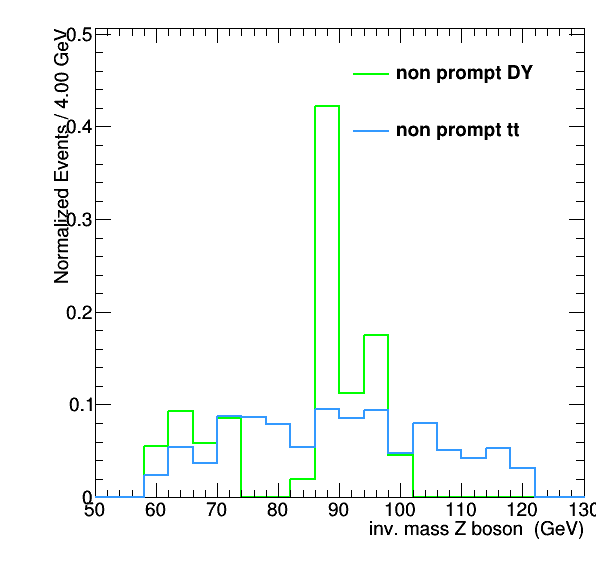
\includegraphics[width=0.47\linewidth]{5_EventSelection/Figures/3lepcontrol_afterAtLeast1Jet_3lep__ZbosonMass_all_Normalized}
	\caption{The normalized distribution for \DY\ and \ttbar+jets events before dividing the events in to regions, after $|\mZ^{\mathrm{reco}} - \mZ| < 30$ GeV. All leptonic channels combined.}
	\label{fig:3lepcontrolafteratleast1jet3lepzbosonmassallnormalized}
\end{figure}
\newpage
\subsection{\TTSR\ and \STSR}
The \TTSR\ is defined to target top quark pair FCNC (\tZq), while the \STSR\ focusses on single top quark FCNC (\tZ). They have \NPL\ contributions coming from \DY\ and \ttbar+jets events. In this region, the data driven \NPL\ template is split into two templates based on the presence of the \NPL\ in the Z boson: 
\begin{itemize}
	\item \NPL\ associated with \PW\ boson is assigned to \DY\ and estimated in the \WZCR.
	\item\NPL\ associated with \PZ\ boson is assigned to \ttbar+jets and estimated in the \TTCR\ and \STCR.
\end{itemize}
%It is shown in \App{app:BDTnp}, that these two templates have the same shape within the limited statistics, not assuming any systematic uncertainties. 

